\subsection{ILASP}\label{sec:ilasp}

\subsubsection{Learning normal rules - learning how to walk}

The first task is learning to walk on the maze, considering adjacent cells and the obstacles (walls and co.). This task have been split for complexity reasons, as a result first it will be learned how to move on near cells and then obstacles will be considered, in 2 different ILASP scripts. Here some normal rules will be learned, other kind of rules have been learned on other scripts but regarding another type of ASP model. 

\subsubsection{Learning to walk on adjacent cells}

This is the ilasp code written for the pourpose, with some bit of background knowledge, definition of search space with language bias and some examples with all the different "cases".  Finding those examples have been pretty difficult because they must be "meaningful" and as such must capture all the different contexts and casistics.

\newpage
\begin{lstlisting}[language=Prolog]
%%%%%%%%%%%%%%%%%%%%%%%%learn how to move on near cells
row(1..5).
col(1..5).

cell(X,Y) :- row(X), col(Y).

succ(0,1).
succ(X, X+1) :- cell(X,_).

%%%%%%%%%%%%%%%%%%%%%%%%%%%%%SEARCH_SPACE + EXAMPLES
#pos(p1, {next((4,2), (4,1)), next((4,2), (4,3)), next((4,2), (3,2)), next((4,2), (5,2))}, {}).
#pos(p2, {next((2,3), (2,2)), next((2,3), (1,3)), next((2,3), (2,4)), next((2,3), (3,3))}, {}).

%no out of range or jump
#neg(a, {next((1,0), (1,1))}, {}).
#neg(b, {next((1,1), (0,1))}, {}).
#neg(c, {next((0,1), (1,1))}, {}).
#neg(d, {next((1,1), (1,0))}, {}).
#neg(e, {next((5,5), (6,5))}, {}).
#neg(f, {next((5,5), (5,6))}, {}).
#neg(g, {next((6,5), (5,5))}, {}).
#neg(h, {next((5,6), (5,5))}, {}).
%no diagonal move
#neg(i, {next((2,4), (1,3))}, {}).
#neg(l, {next((2,4), (1,5))}, {}).
#neg(m, {next((2,4), (3,5))}, {}).
#neg(n, {next((2,4), (3,3))}, {}).
%no move same cell
#neg(o, {next((2,4), (2,4))}, {}).

#modeb(2, cell(var(r), var(c)), (positive, anti_reflexive)).
#modeb(1, succ(var(c), var(c)), (positive, anti_reflexive)).
#modeb(1, succ(var(r), var(r)), (positive, anti_reflexive)).
#modeh(next((var(r), var(c)), (var(r), var(c)))).

#maxv(3).
\end{lstlisting}

Successor predicate have been inserted, it rapresent the simple "arithmetic" concept of successive numbers, it's important to define because ILASP doesn't include this "sum" operator bilt-in.
In the language bias definition I used the "positive" and "anti-reflexive" options to reduce the search-space and found earlier the result. This options could be avoided.
At \ref{fig:asd} the output of the script, with the learned rules, ILASP actually learned that "next" predicate is true for adjacent cells, based on that the movement on the grid will be possible.
NB: this is equivalent to the predicate "adjacent" learned by my companions
\begin{figure}
	\centering
	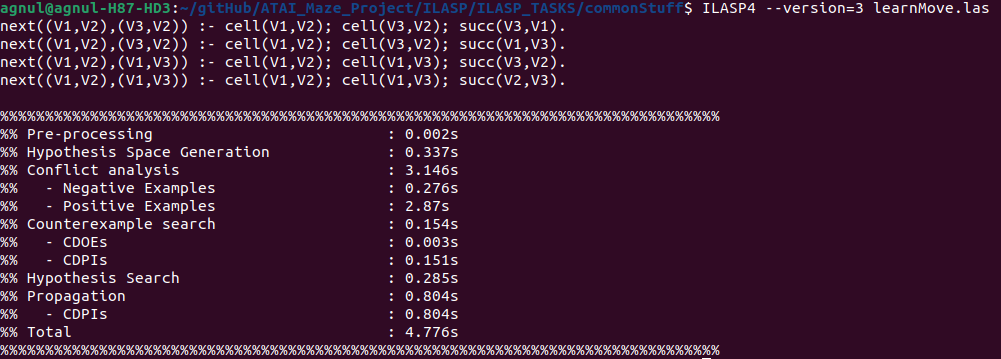
\includegraphics[scale=0.5]{img/learnMoveAdj.png}
	\caption{Learned rules - adjacent move}\label{fig:asd}
\end{figure}

\newpage
\subsubsection{Learning to walk on cells without obstacles}
The next step is to consider obstacles on the grid, as discussed in the Introduction part of the report. Here the goal is to find a new normal rule that represent the concet of a "valid move", in a cell without obstacles.
Initially, a maze is defined, this is the same maze used by my companions for our work.
This is the task written for the purpose:
\newpage

\begin{lstlisting}[language=Prolog]
%%%%%%%%%%%%%%%%%%%%%%%%%%%%%%learn how to move on cells without obstacles
row(1..5).
col(1..5).

obstacle(1,2).
obstacle(2,2).
obstacle(3,2).
obstacle(3,3).
obstacle(4,3).
obstacle(4,4).
obstacle(3,4).
obstacle(2,4).
obstacle(1,4).
obstacle(1,5).
obstacle(5,1).

start(1,1).
goal(5,5).

%%%%%%%%%%%%%%

cell(X,Y) :- row(X), col(Y).

succ(0,1).
succ(X, X+1) :- cell(X,_).

%PATHS ADJACENTS (learned from previous ilasp task)
next((V1,V2),(V3,V2)) :- cell(V1,V2), cell(V3,V2), succ(V3,V1).
next((V1,V2),(V3,V2)) :- cell(V1,V2), cell(V3,V2), succ(V1,V3).
next((V1,V2),(V1,V3)) :- cell(V1,V2), cell(V1,V3), succ(V3,V2).
next((V1,V2),(V1,V3)) :- cell(V1,V2), cell(V1,V3), succ(V2,V3).


%%%%%%%%%%%%%%%%%%%%%%%%%%%%%SEARCH_SPACE + EXAMPLES

#pos(po, {nextLegit((1,1),(2,1))}, {}).
#pos(po2, {nextLegit((4,1),(4,2))}, {}).

%no movement on obstacles
#neg(a, {nextLegit((1,1),(1,2))}, {}).
#neg(av, {nextLegit((3,2),(4,2))}, {}).
#neg(af, {nextLegit((1,2),(1,1))}, {}).
#neg(b, {nextLegit((4,1),(5,1))}, {}).
#neg(g, {nextLegit((3,3),(2,3))}, {}).

#modeb(1, next((var(r), var(c)), (var(r), var(c)))).
#modeb(2, obstacle(var(r), var(c))).
#modeh(1, nextLegit((var(r), var(c)), (var(r), var(c)))).

#maxv(3).
\end{lstlisting}
In the code the rules learned previously have been inserted and used in the search space. 
Negative examples shows that no movement is possible TO obstacles and FROM obstacles, this 2 casistics are important for a correct learning.
At \ref{fig:asd2} the output of the script, with the learned rules, ILASP actually learned this new "nextLegit" predicate that represent the concept of a valid move: a move from (or to) cells without obstacles.

NB: this is equivalent to the "move" predicate learned by my companions.
\begin{figure}
	\centering
	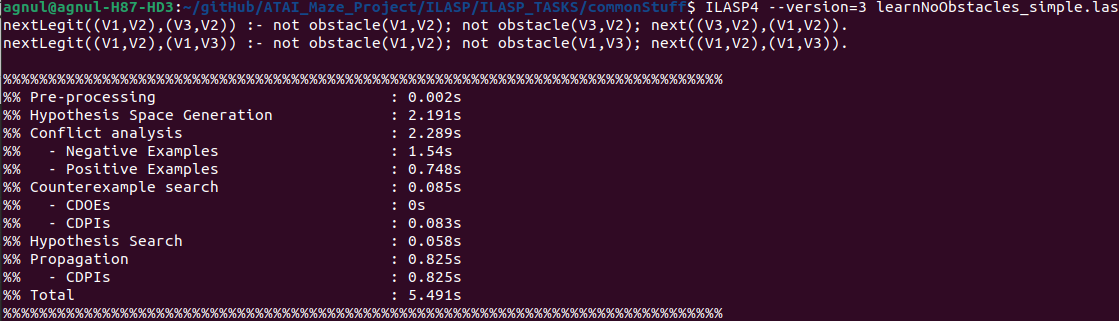
\includegraphics[scale=0.45]{img/learn_noObstacles.png}
	\caption{Learned rules - avoid obstacles}\label{fig:asd2}
\end{figure}


\newpage
It's interesting to see that, setting 3 variables in the language bias, ilasp learned just 2 rules: it considers the cases when near cells share the same horizontal or vertical direction. 
Probably, I would have write 4 rules using 4 different variables in a naive way, considering the "4 directions adjacency", but this tool finds a more compact solution.
\subsubsection{using this rules to define an ASP model}
having this rules in hand now is possible to define a model that solves our problem. Learned rules are reported exactly as they were on the ILASP scripts output. Some pieces are missing: some other rules need to be defined but they are quite intiuitive at this point. The maze reported on the encoding is the same used for the ilasp task.
 
 \newpage
\begin{lstlisting}[language=Prolog]
	%MODEL THAT SOLVES PROBLEM OF PATHFINDING IN THE GRID
	row(1..5).
	col(1..5).
	
	obstacle(1,2).
	obstacle(2,2).
	obstacle(3,2).
	obstacle(4,4).
	obstacle(3,4).
	obstacle(2,4).
	obstacle(1,4).
	obstacle(1,5).
	obstacle(5,1).
	
	start(1,1).
	goal(2,5).
	
	%for each position define cell pred.
	cell(X,Y) :- row(X), col(Y).
	
	%FIND A PATH FROM START
	move(0,0,X,Y) :- start(X,Y).
	%for each "move" find another linked to it that is a legit move!
	1{move(X,Y,X1,Y1): nextLegit((X,Y), (X1,Y1))}1:- move(_,_, X,Y), not goal(X,Y).
	
	succ(0,1).
	succ(X, X+1) :- cell(X,_).
	
	%LEARNED BY ILASP, move on adj cells.
	next((V1,V2),(V3,V2)) :- cell(V1,V2), cell(V3,V2), succ(V3,V1).
	next((V1,V2),(V3,V2)) :- cell(V1,V2), cell(V3,V2), succ(V1,V3).
	next((V1,V2),(V1,V3)) :- cell(V1,V2), cell(V1,V3), succ(V3,V2).
	next((V1,V2),(V1,V3)) :- cell(V1,V2), cell(V1,V3), succ(V2,V3).
	
	%LEARNED BY ILASP, move on adj cells. without obstacles
	nextLegit((V1,V2),(V3,V2)) :- not obstacle(V1,V2); not obstacle(V3,V2); next((V3,V2),(V1,V2)).
	nextLegit((V1,V2),(V1,V3)) :- not obstacle(V1,V2); not obstacle(V1,V3); next((V1,V2),(V1,V3)).
	
	%ON GOAL POSITION STOP
	:- goal(X,Y), not move(_,_, X,Y).
	
	#show move/4.
\end{lstlisting}

at \ref{fig:asd3} the execution of "clingo" command on this model is shown: the path is represented by the chaning "move" predicate.

\newpage
\begin{figure}
	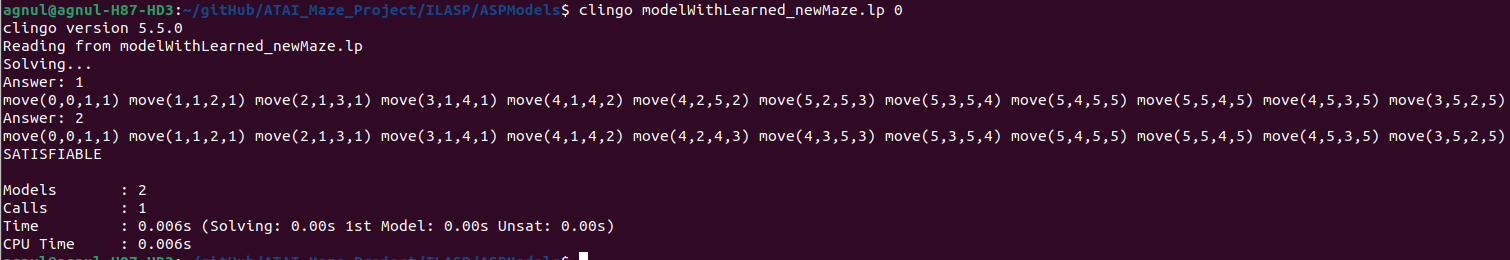
\includegraphics[scale=0.3]{img/outputModel_newMaze.png}
	\caption{Path found on the grid}\label{fig:asd3}
\end{figure}

\subsubsection{performance test - scalability}
The work done with ilasp shows clearly this fact: the time complexity doesn't scale well with respect to the search space dimension. In fact, when trying to learn the "move to adjacent cells AND without obstacles" (the 2 tasks on the same scrit) compexity costs exploded "simply" for the insertion of the predicate "obstacle". (for a total of 6 predicates in the search space). it is quite evident that a sort of exponential trend is in place and here I will like to do a specific test to demonstrate this.

Using the "learn to walk on adjacent cells" ilasp script I tried to augment the search space and see time needed for computation, the augmenting has been done insertig other predicates in language bias, modyfing language bias to insert more "usage" of the same predicate, eliminating the "positive" and "anti-reflexing" options on language bias. After that, an analysis on computation time vs search space dimension (measured as the size of rules in the search space) has been conducted, at \ref{fig:asd4} the graphical results, the blue points are the instantes of the benchmarks. Interestingly other tests conducted with a searh space grater than 200 lead to huge times like 2 hours.

The grow shows an evident simil-exponential trend, especially the steep from the "57 seconds" point to the "200" one.
\newpage

\begin{figure}
	\centering
	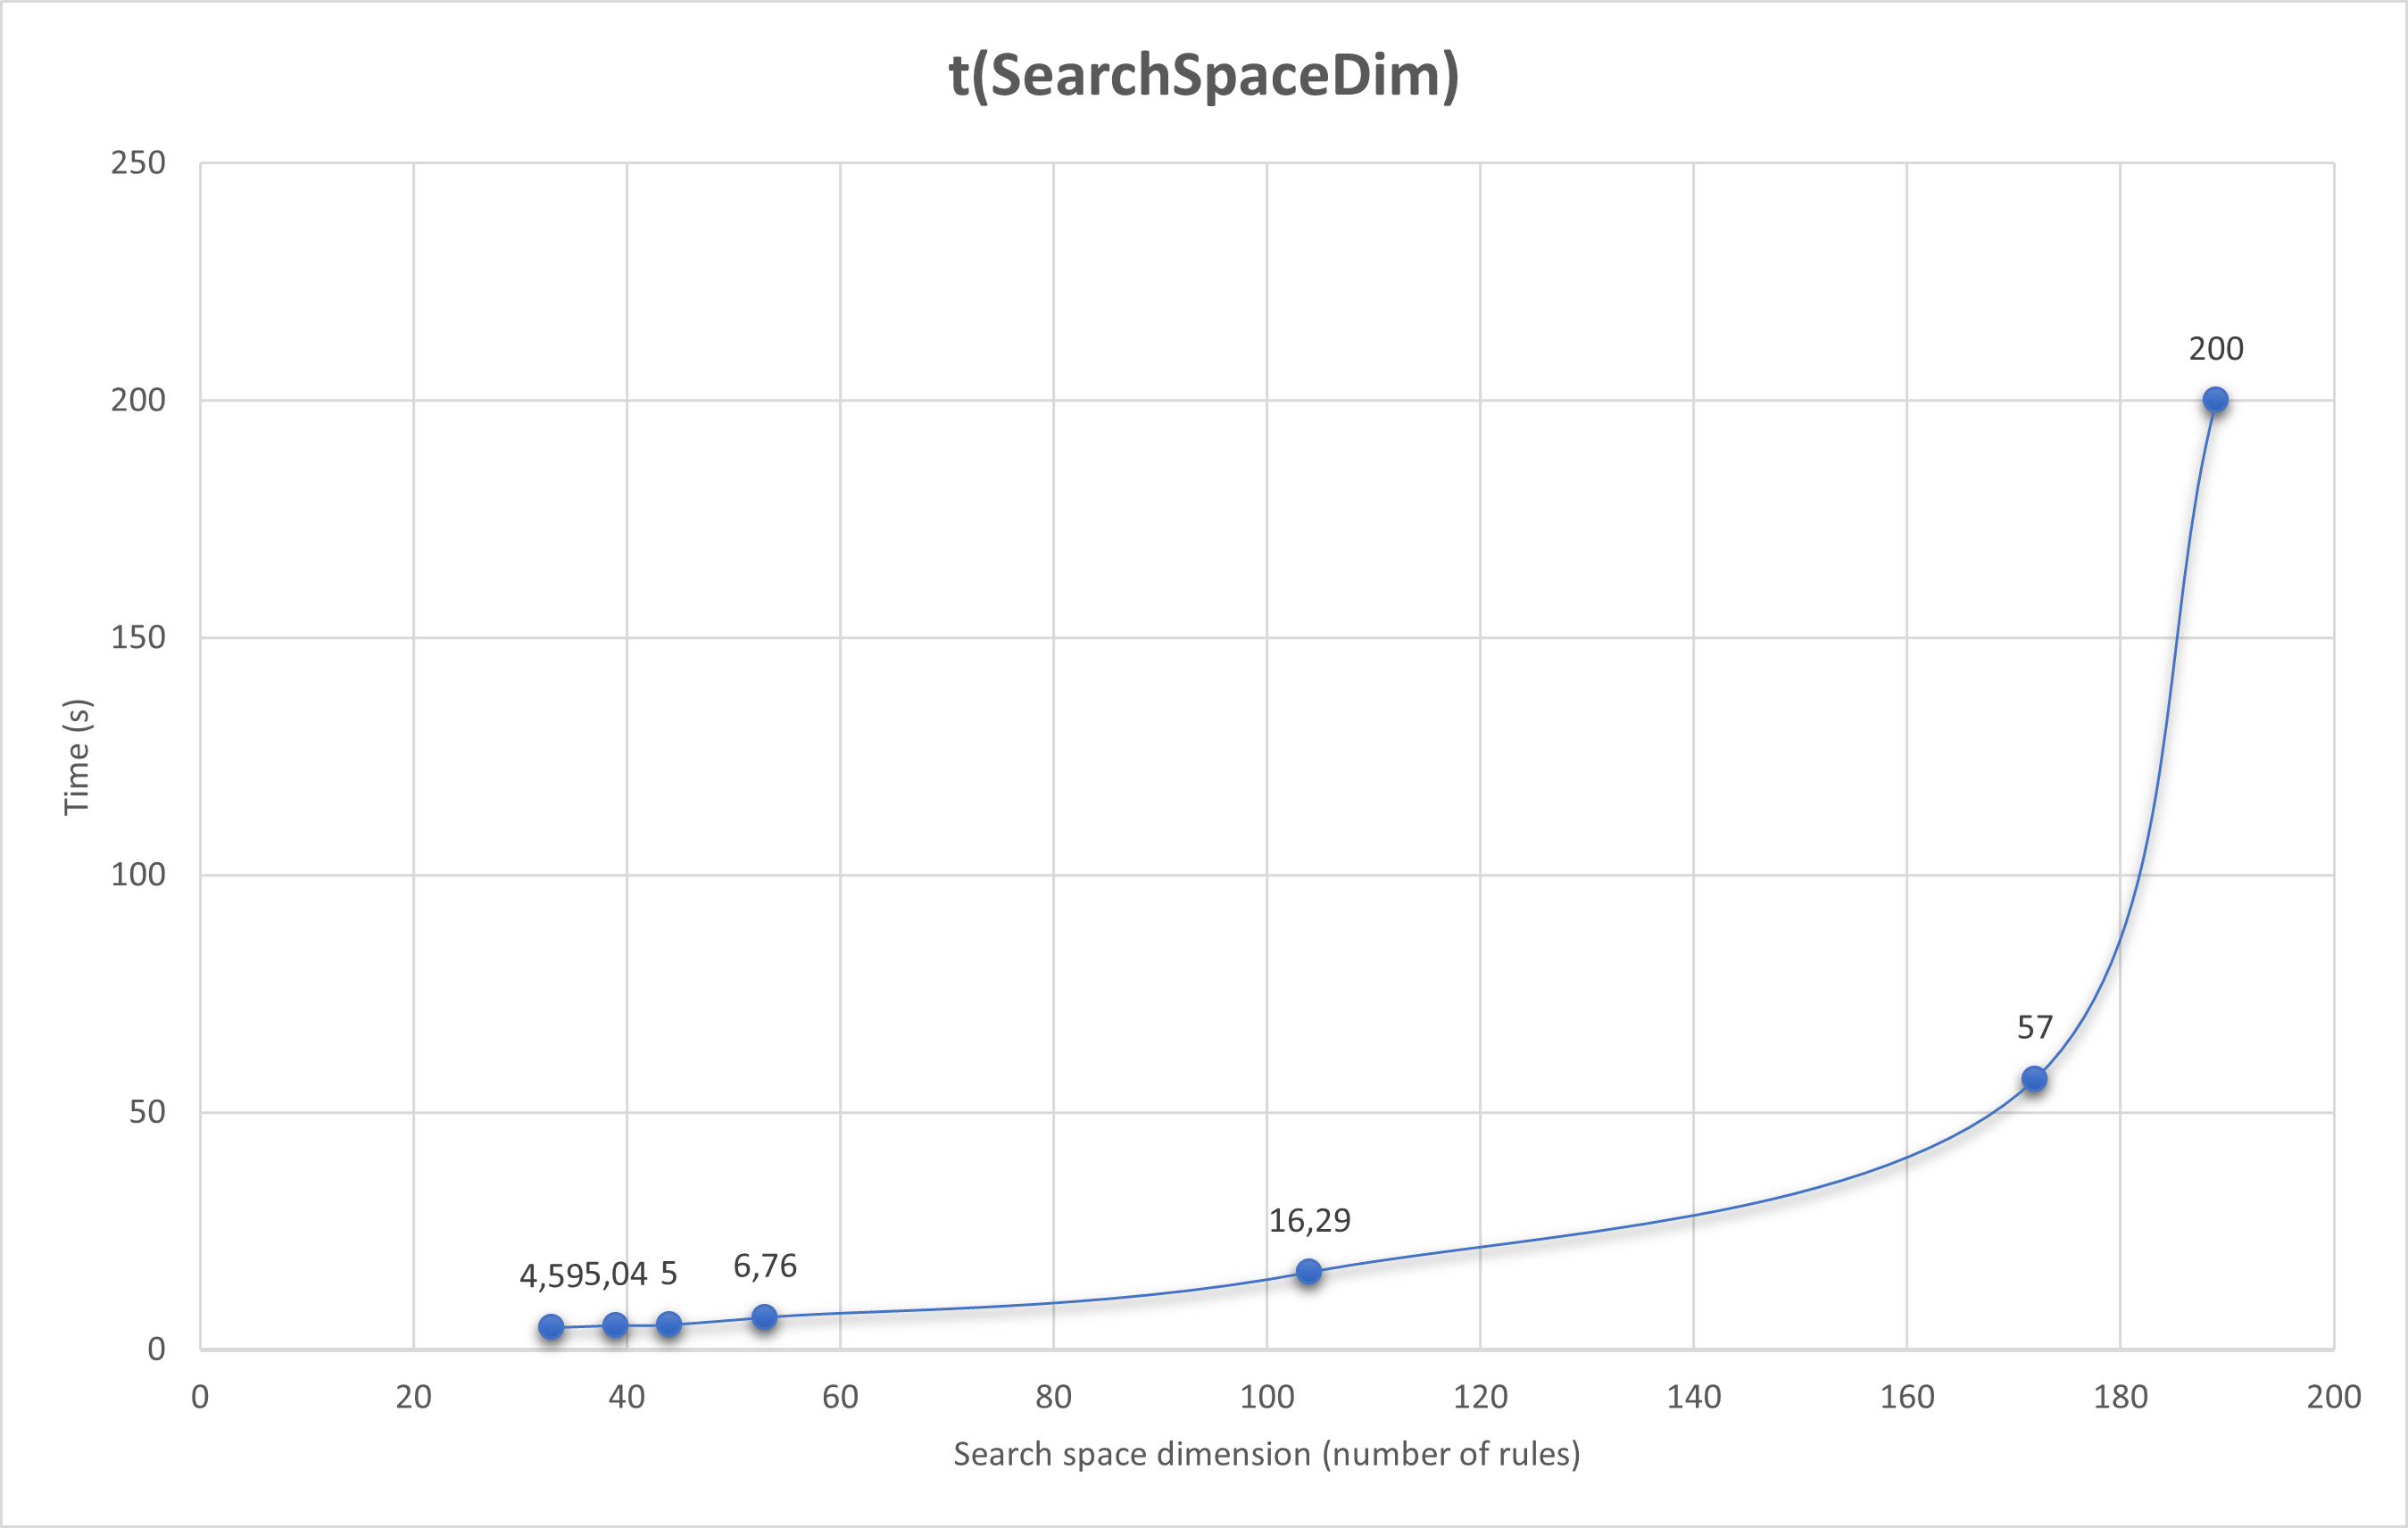
\includegraphics[scale=0.7]{img/GraphTimes.png}
	\caption{performance test result}\label{fig:asd4}
\end{figure}



\newpage